\iffalse
\documentclass[journal,12pt,twocolumn]{IEEEtran}
\usepackage{cite}
\usepackage{amsmath,amssymb,amsfonts,amsthm}
\usepackage{algorithmic}
\usepackage{graphicx}
\usepackage{textcomp}
\usepackage{xcolor}
\usepackage{txfonts}
\usepackage{listings}
\usepackage{enumitem}
\usepackage{mathtools}
\usepackage{float}
\usepackage{gensymb}
\usepackage{comment}
\usepackage[breaklinks=true]{hyperref}
\usepackage{tkz-euclide} 
\usepackage{listings}
\usepackage{gvv}                                        
\def\inputGnumericTable{}                                 
\usepackage[latin1]{inputenc}                                
\usepackage{color}                                            
\usepackage{array}                                            
\usepackage{longtable}                                       
\usepackage{calc}                                             
\usepackage{multirow}                                         
\usepackage{hhline}                                           
\usepackage{ifthen}                                           
\usepackage{lscape}
\usepackage{amsmath}
\newtheorem{theorem}{Theorem}[section]
\newtheorem{problem}{Problem}
\newtheorem{proposition}{Proposition}[section]
\newtheorem{lemma}{Lemma}[section]
\newtheorem{corollary}[theorem]{Corollary}
\newtheorem{example}{Example}[section]
\newtheorem{definition}[problem]{Definition}
\newcommand{\BEQA}{\begin{eqnarray}}
\newcommand{\EEQA}{\end{eqnarray}}
\newcommand{\define}{\stackrel{\triangle}{=}}
\theoremstyle{remark}
\newtheorem{rem}{Remark}

\usepackage{circuitikz} 

\begin{document}

\bibliographystyle{IEEEtran}
\vspace{3cm}

\title{NCERT Analog- 12.7.7}
\author{EE23BTECH11045 - Palavelli Srija$^{*}$}

\maketitle

\bigskip

\renewcommand{\thefigure}{\theenumi}
\renewcommand{\thetable}{\theenumi}

\vspace{3cm}
\textbf{Question 12.7.7:} 
 A charged $30 \mu F$ capacitor is connected to a $27 mH$ inductor. What is the angular frequency of free oscillations of the circuit?\\
\textbf{Solution: }
\fi
\begin{table}[h!]
    \centering
    
    \begin{tabular}{|c|l|c|}
        \hline
        \textbf{Symbol} & \textbf{Description} & \textbf{Value} \\
        \hline
        \(C\) & Capacitance & \(30 \mu F\) \\
        \(L\) & Inductance & \(27 mH\) \\
        \(\omega_0\) & Angular Frequency & ??\\
        \hline
    \end{tabular}

    \caption{Input Parameters}
    \label{tab:table_omega}
\end{table}
\begin{figure}[H]
    \centering
    \begin{circuitikz}
   \draw(0, 0) to [L, l=$27\,\text{mH}$] (0, -2);
   
    \draw(0, 0) -- (3, 0);
   \draw(3, 0) to [C, l=$30\,\mu\text{F}$] (3, -2) -- (0, -2);
 \draw (2, 0) -- (3, 0) node[midway, below] {-};
    \draw (2, -2) -- (3, -2) node[midway, above] {+};
    \draw (-0.5, 0) node[ below] {+};
    \draw (-0.5, -2) node[above] {-};
 \draw (-0.25, -1) node[left] {$V_L$};
    % Draw current arrow
   \draw[<-] (1, 0) -- (2, 0) node[midway, above] {$I(t)$};
   \draw (2.5, -1) node[left] {$V_C$};
\end{circuitikz}


    \caption{LC Circuit Diagram}
    \label{fig:sr33}
\end{figure}
at $t=0^-\quad V_C=-V_0,\quad I(0)=0,\quad V_L=V_0$\\

\begin{figure}[H]
    \centering
    
\begin{circuitikz}
\tikzstyle{every node}=[font=\Large]
\draw (6.75,13.5) to[L,l={ \LARGE $sL$} ] (6.75,10.75);
\draw [](6.75,13.5) to[short] (10.75,13.5);
\draw [](6.75,10.75) to[short] (10.75,10.75);
\draw (10.75,13.5) to[C,l={ \LARGE $1/sC$}] (10.75,12);
\draw (10.75,12) to[american voltage source,l={ \LARGE $V_0/s$}] (10.75,10.75);
\draw [->, >=Stealth] (8.5,13.5) -- (8.25,13.5);
\draw (8.5,13.5) -- (8.25,13.5) node[midway, above] {$I(s)$};
\end{circuitikz}


   \caption{LC Circuit Diagram in S domain}
    \label{fig:sr32}
\end{figure}
\begin{align}
sL I(s) + \frac{1}{sC} I(s) &= \frac{V_0}{s} \\
I(s) &= \frac{V_0C}{s^2LC + 1} \\
\mathcal{L}^{-1}\{I(s)\} &= I(t) \\
I(t) &= \frac{V_0C}{\sqrt{LC}} \sin\left(t\frac{1}{\sqrt{LC}}\right) \\
I(t) &= V_0\sqrt{\frac{C}{L}} \sin\left(t\frac{1}{\sqrt{LC}}\right)
\end{align}

Net impedence of LC circuit \\
\begin{align}
Z&=R_L +R_C \\
&=Ls + \dfrac{1}{sC} 
\end{align}
At resonance, the resistance of capacitor and inductor cancel out as follows:
\begin{align}
    Ls + \dfrac{1}{sC} &= 0\\
    \implies s &= j\dfrac{1}{\sqrt{LC}} \label{eq:sr20}
\end{align}
$s$ can be expressed in terms of angular resonance frequency as
\begin{equation}
    s = j\omega_0 \label{eq:sr21}
\end{equation}
on comparing \eqref{eq:sr20} and \eqref{eq:sr21}
\begin{equation}
    \omega_0 = \dfrac{1}{\sqrt{LC}}
\end{equation}
\begin{align}
\omega_0 &= \frac{1}{\sqrt{(30 \times 10^{-6}) \times (27 \times 10^{-3})}} \\
&= \frac{1}{\sqrt{8.1 \times 10^{-7}}}\\
& \approx 1.11 \times 10^{3} \, \text{rad/s}
\end{align}
Assuming $V_0=1$volt\\
\begin{figure}[h!]
    \centering
    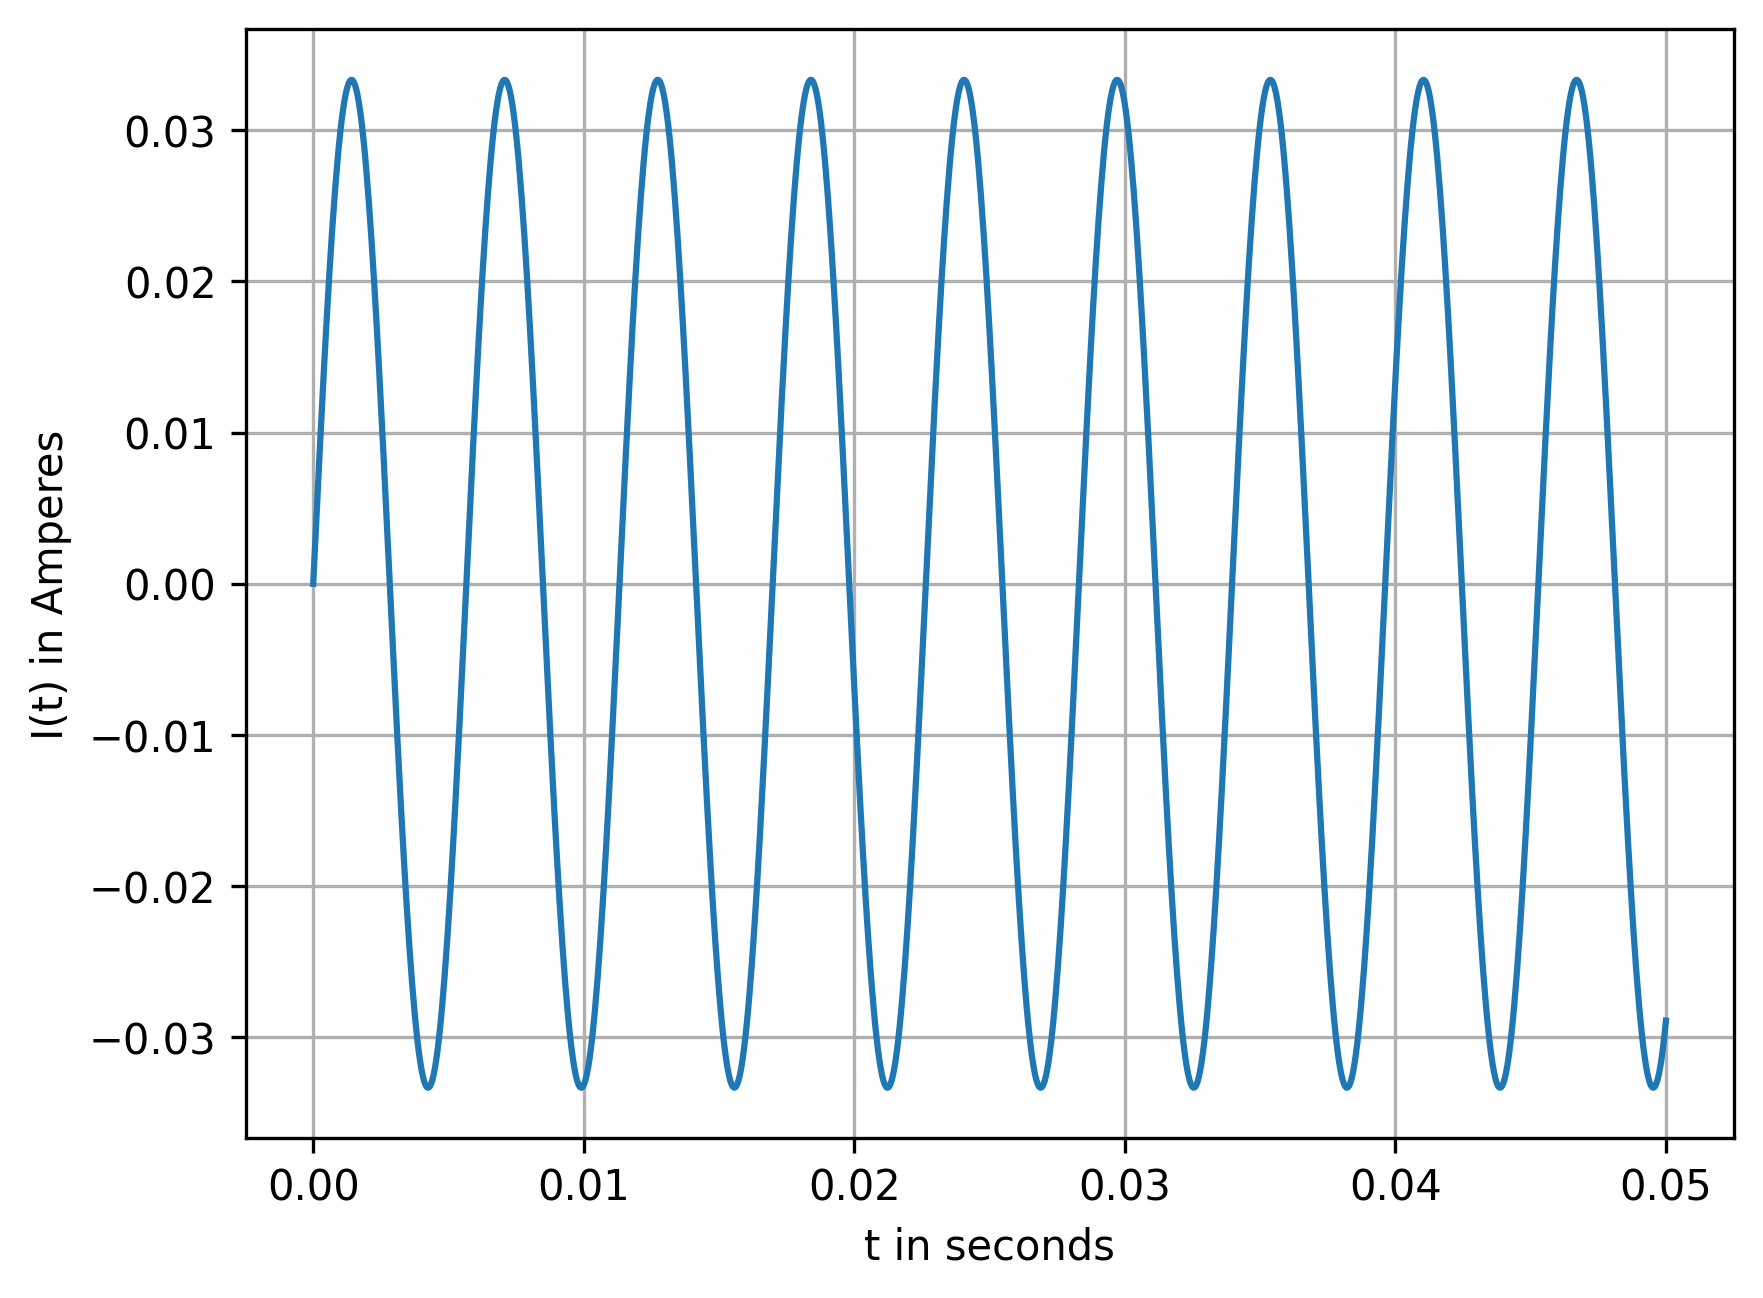
\includegraphics[width=\columnwidth,height=5cm]{ncert-physics/12/7/7/figs/p.png}
    \caption{I(t) vs t}
    \label{fig:sr31}
\end{figure}
%\end{document}

